\section{Referencia de la Clase Factura\-Proveedor\-View}
\label{classFacturaProveedorView}\index{FacturaProveedorView@{FacturaProveedorView}}
Muestra y administra la ventana de factura de proveedor.  


{\tt \#include $<$facturapview.h$>$}

Diagrama de herencias de Factura\-Proveedor\-View\begin{figure}[H]
\begin{center}
\leavevmode
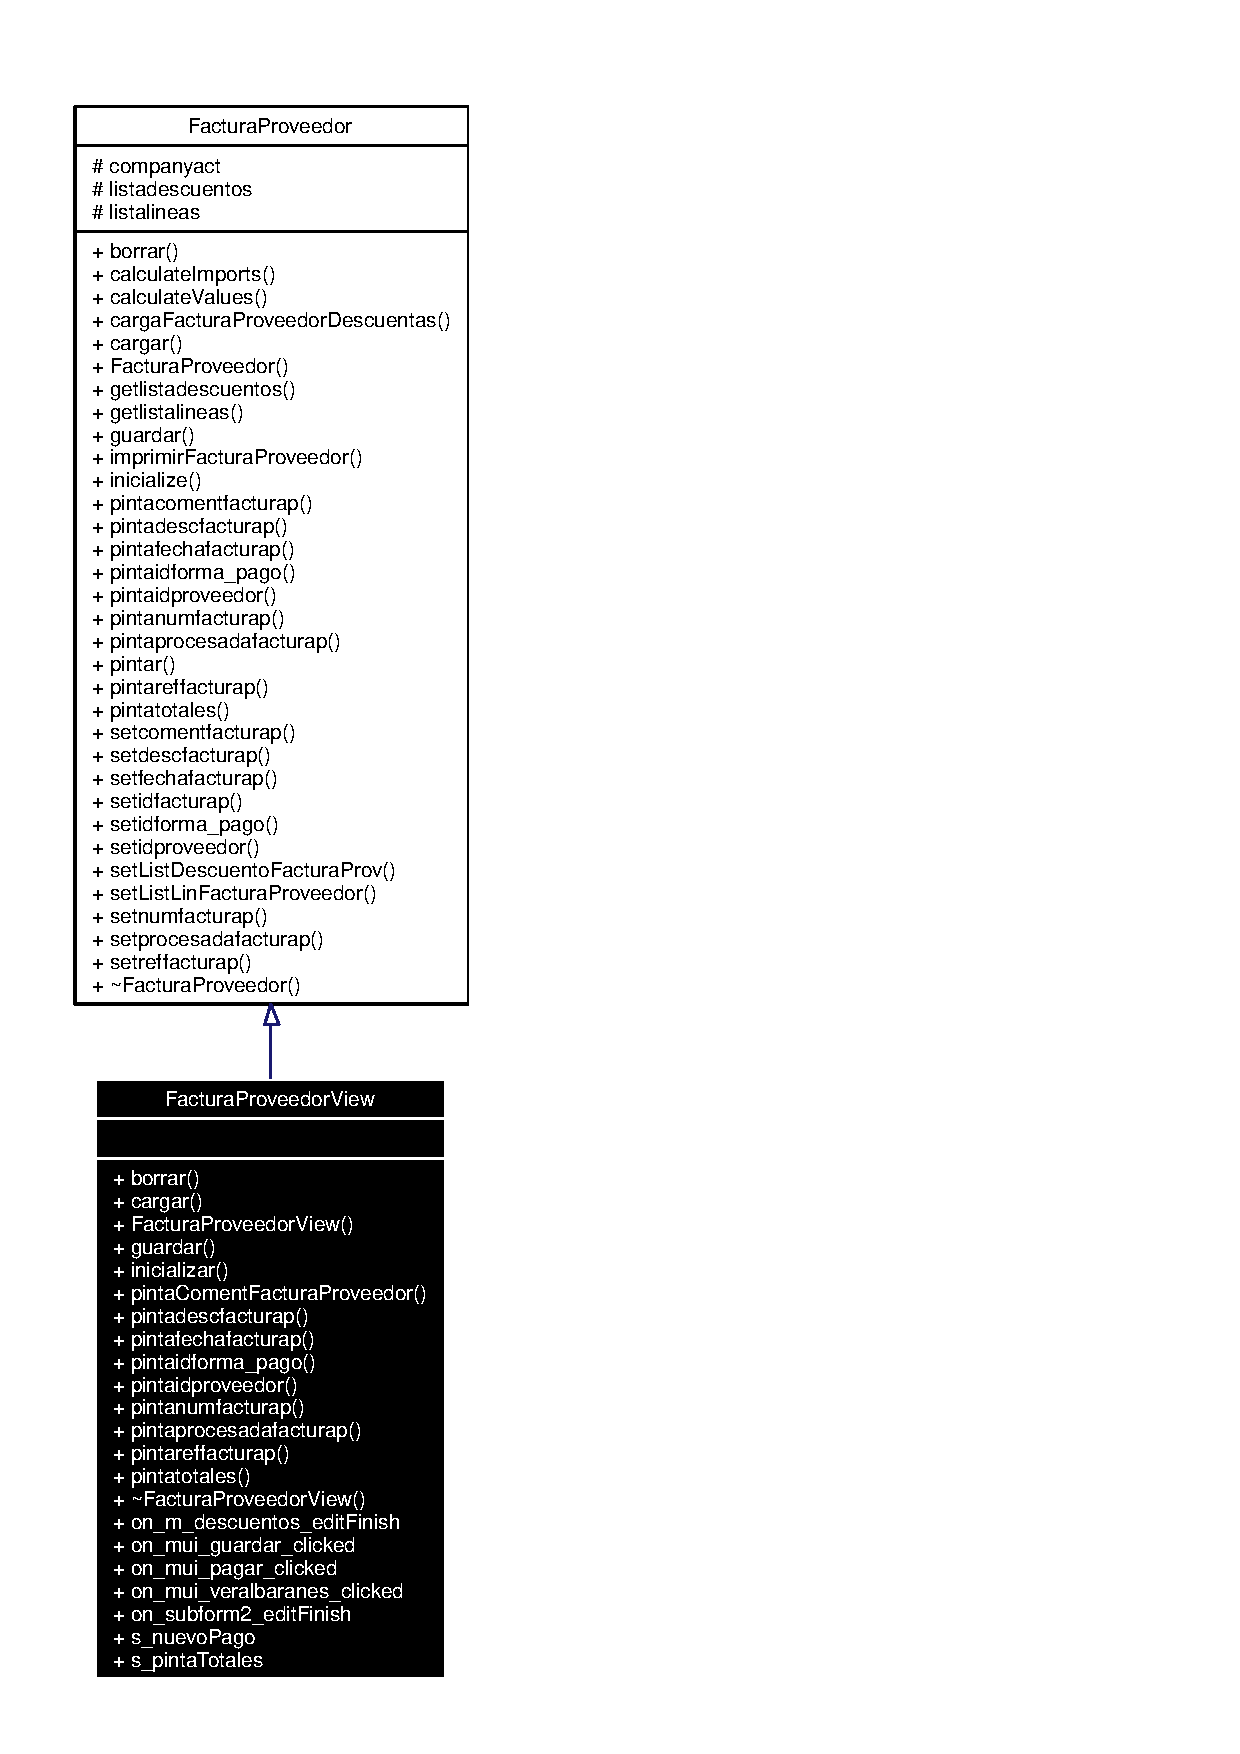
\includegraphics[width=112pt]{classFacturaProveedorView__inherit__graph}
\end{center}
\end{figure}
Diagrama de colaboraci\'{o}n para Factura\-Proveedor\-View:\begin{figure}[H]
\begin{center}
\leavevmode
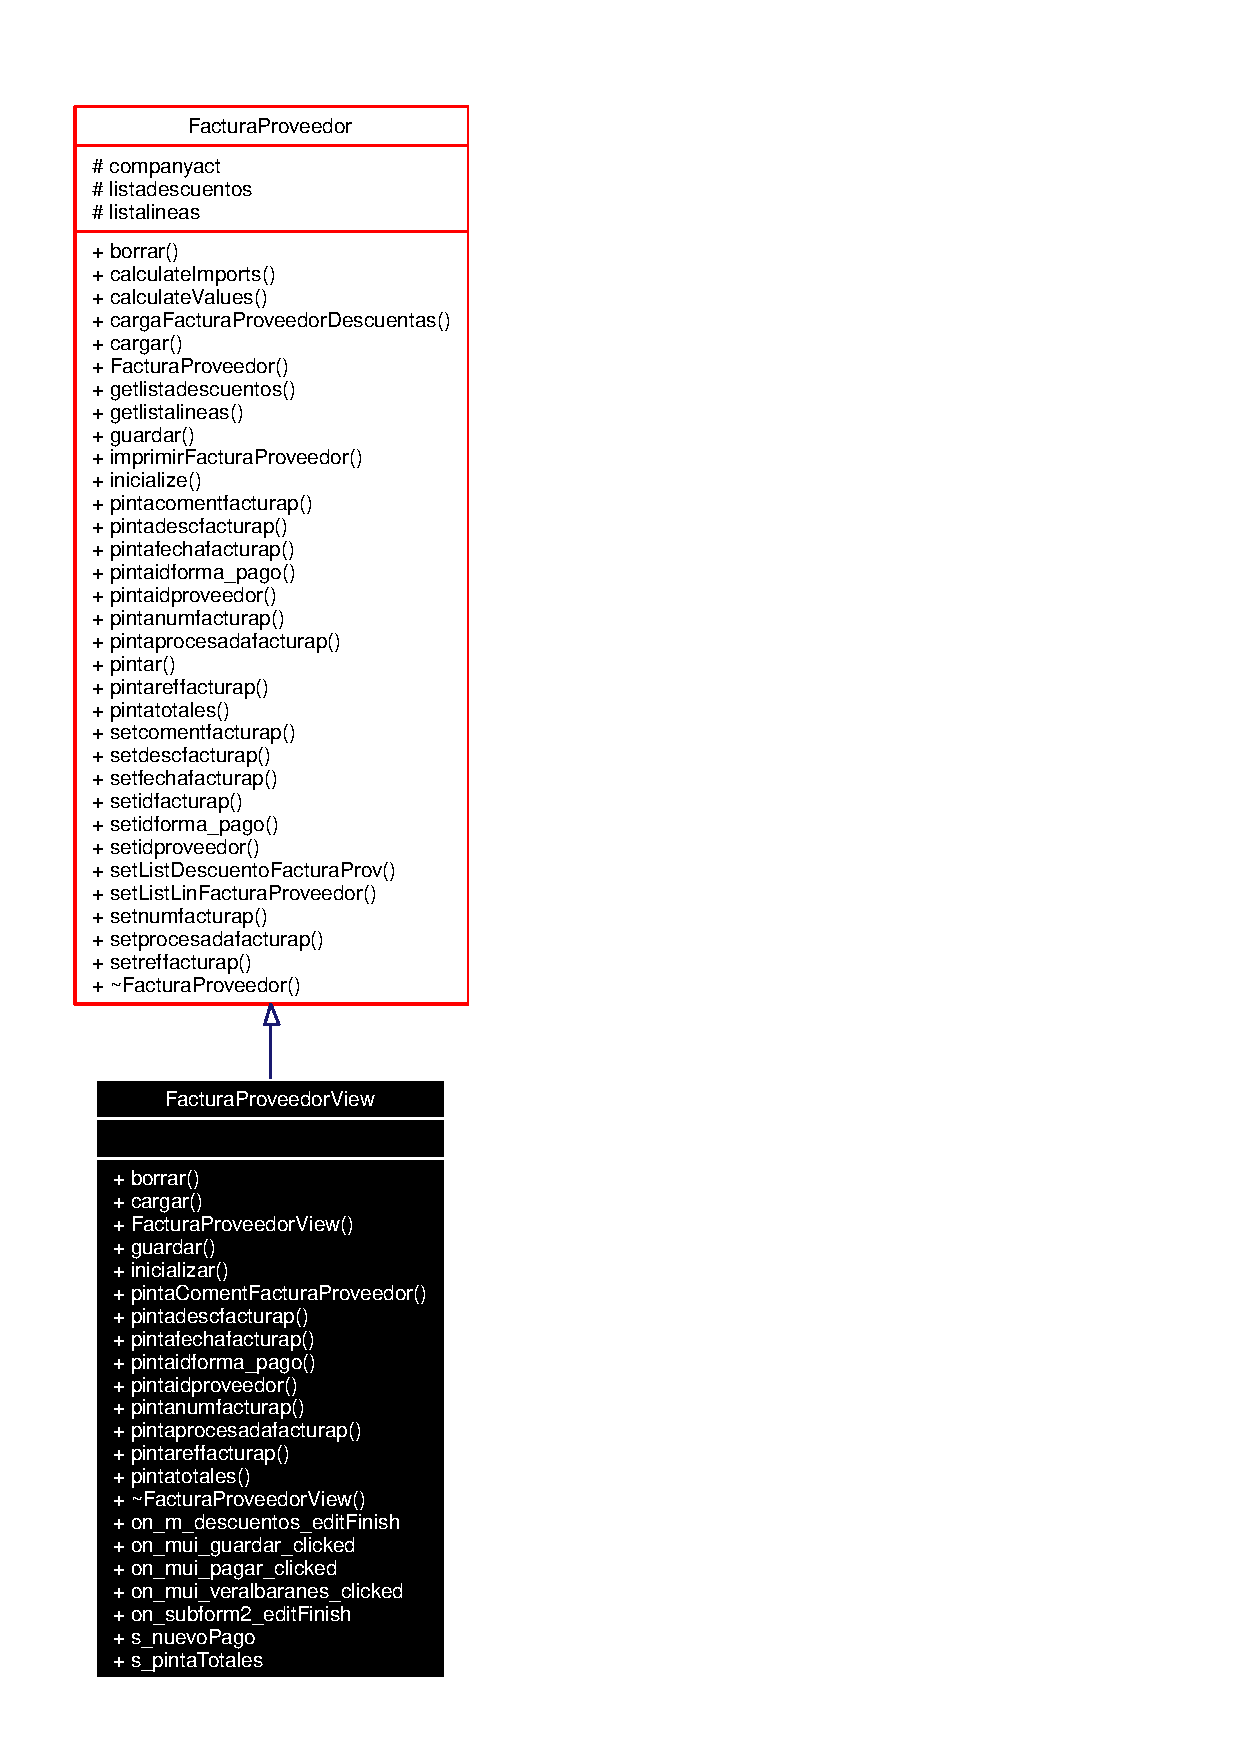
\includegraphics[width=112pt]{classFacturaProveedorView__coll__graph}
\end{center}
\end{figure}
\subsection*{Slots p\'{u}blicos}
\begin{CompactItemize}
\item 
virtual void {\bf on\_\-m\_\-descuentos\_\-edit\-Finish} (int, int)\label{classFacturaProveedorView_i0}

\item 
virtual void {\bf on\_\-mui\_\-guardar\_\-clicked} ()\label{classFacturaProveedorView_i1}

\item 
virtual void {\bf on\_\-mui\_\-pagar\_\-clicked} ()\label{classFacturaProveedorView_i2}

\item 
virtual void {\bf on\_\-mui\_\-veralbaranes\_\-clicked} ()\label{classFacturaProveedorView_i3}

\item 
virtual void {\bf on\_\-subform2\_\-edit\-Finish} (int, int)\label{classFacturaProveedorView_i4}

\item 
virtual void {\bf s\_\-nuevo\-Pago} ()\label{classFacturaProveedorView_i5}

\item 
virtual void {\bf s\_\-pinta\-Totales} ()\label{classFacturaProveedorView_i6}

\begin{CompactList}\small\item\em Este slot se activa cuando hay cambios en los subformularios. \item\end{CompactList}\end{CompactItemize}
\subsection*{M\'{e}todos p\'{u}blicos}
\begin{CompactItemize}
\item 
virtual int {\bf borrar} ()\label{classFacturaProveedorView_a0}

\item 
virtual int {\bf cargar} (QString id)\label{classFacturaProveedorView_a1}

\begin{CompactList}\small\item\em Esta funcion carga un {\bf Factura\-Proveedor}{\rm (p.\,\pageref{classFacturaProveedor})}. \item\end{CompactList}\item 
{\bf Factura\-Proveedor\-View} ({\bf company} $\ast$, QWidget $\ast$parent=0)
\item 
virtual int {\bf guardar} ()\label{classFacturaProveedorView_a3}

\begin{CompactList}\small\item\em Estos metodos deben existir para poder trabajar con la clase Ficha. \item\end{CompactList}\item 
void {\bf inicializar} ()
\item 
void {\bf pinta\-Coment\-Factura\-Proveedor} (QString id)\label{classFacturaProveedorView_a5}

\item 
void {\bf pintadescfacturap} (QString id)\label{classFacturaProveedorView_a6}

\item 
void {\bf pintafechafacturap} (QString id)\label{classFacturaProveedorView_a7}

\item 
void {\bf pintaidforma\_\-pago} (QString id)\label{classFacturaProveedorView_a8}

\item 
void {\bf pintaidproveedor} (QString id)\label{classFacturaProveedorView_a9}

\item 
void {\bf pintanumfacturap} (QString id)\label{classFacturaProveedorView_a10}

\item 
void {\bf pintaprocesadafacturap} (QString id)\label{classFacturaProveedorView_a11}

\item 
void {\bf pintareffacturap} (QString id)\label{classFacturaProveedorView_a12}

\item 
virtual void {\bf pintatotales} (Fixed base, Fixed iva)\label{classFacturaProveedorView_a13}

\end{CompactItemize}


\subsection{Descripci\'{o}n detallada}
Muestra y administra la ventana de factura de proveedor. 



\subsection{Documentaci\'{o}n del constructor y destructor}
\index{FacturaProveedorView@{Factura\-Proveedor\-View}!FacturaProveedorView@{FacturaProveedorView}}
\index{FacturaProveedorView@{FacturaProveedorView}!FacturaProveedorView@{Factura\-Proveedor\-View}}
\subsubsection{\setlength{\rightskip}{0pt plus 5cm}Factura\-Proveedor\-View::Factura\-Proveedor\-View ({\bf company} $\ast$ {\em comp}, QWidget $\ast$ {\em parent} = {\tt 0})}\label{classFacturaProveedorView_a2}


Usurpamos la identidad de mlist y ponemos nuestro propio widget con sus cosillas. 

\subsection{Documentaci\'{o}n de las funciones miembro}
\index{FacturaProveedorView@{Factura\-Proveedor\-View}!inicializar@{inicializar}}
\index{inicializar@{inicializar}!FacturaProveedorView@{Factura\-Proveedor\-View}}
\subsubsection{\setlength{\rightskip}{0pt plus 5cm}void Factura\-Proveedor\-View::inicializar ()}\label{classFacturaProveedorView_a4}


inicializar debe ser invocado cuando se crea una nueva ficha sin cargar ningun date de la base de datos (por ejemplo una nueva ficha). Sirve para inicializar los componenetes sin necesidad de query alguno 

La documentaci\'{o}n para esta clase fu\'{e} generada a partir de los siguientes archivos:\begin{CompactItemize}
\item 
facturapview.h\item 
facturapview.cpp\end{CompactItemize}
